\subsection{添加}

设 E 是域 K 的一个扩张。给定一族 E 中的元素 \(\mathbf{x} = (x_{i})_{i \in I}\)，我们用 \(\mathrm{K}(x_{i})_{i \in I}\)（或 \(\mathrm{K}(\mathbf{x})\)，或也记作 \(\mathrm{K}(x_{1}, \ldots, x_{n})\)，当 I 是 N 中的区间 {[}1, n{]} 时）表示包含该族成员 \((x_{i})\) 的最小子扩张；我们说 \(\mathrm{K}(x_{i})_{i\in I}\) 是通过把族 \((x_{i})_{i\in I}\) 中的元素添加到 K 上而得到的，并且该族 \((x_{i})_{i\in I}\)（或其元素的集合）是 \(\mathrm{K}(x_{i})_{i\in I}\) 关于 K（或在 K 上）的生成族。域 \(\mathrm{K}(x_{i})_{i\in I}\) 仅依赖于族 \((x_{i})_{i\in I}\) 的元素集合 A；我们也把它记作 \(\mathrm{K}(\mathrm{A})\) 。特别地，我们有 \(\mathrm{K}(\mathrm{E})=\mathrm{E}\) 且 \(\mathrm{K}(\emptyset)=\mathrm{K} \cdot 1\) 。以上所述特别适用于 E 为包含 K 作为子域的域的情形。

\pandocbounded{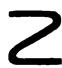
\includegraphics[keepaspectratio]{images/part001_724f36f3.jpg}}

应当注意，A 一般不构成代数 \(\mathbf{K}(\mathbf{A})\) 的生成集，换言之，\(\mathbf{K}(\mathbf{A}) \neq \mathbf{K}[\mathbf{A}]\) 。* 然而我们将看到，\(\mathbf{K}(\mathbf{A}) = \mathbf{K}[\mathbf{A}]\)（当 \(\mathbf{K}(\mathbf{A})\) 是 \(\mathbf{K}\) 的一个代数扩张时；V，第 18 页，推论 1）。*

命题 2. --- 若 M 和 N 是域 K 的一个扩张中的任意两个子集，则 \(\mathbf{K}(\mathbf{M} \cup \mathbf{N}) = \mathbf{K}(\mathbf{M})(\mathbf{N}) = \mathbf{K}(\mathbf{N})(\mathbf{M})\) 。

因为 \(\mathbf{K}(\mathbf{M} \cup \mathbf{N})\) 包含 \(\mathbf{K}(\mathbf{M})\) 与 \(\mathbf{N}\)，因此包含 \(\mathbf{K}(\mathbf{M})(\mathbf{N})\)；由于 \(\mathbf{K}(\mathbf{M})(\mathbf{N})\) 是一个包含 \(\mathbf{K} \cup \mathbf{M} \cup \mathbf{N}\) 的域，它包含 \(\mathbf{K}(\mathbf{M} \cup \mathbf{N})\)，由此得出该命题。

我们有时会写 \(\mathbf{K}(\mathbf{M},\mathbf{N})\) 以代替 \(\mathbf{K}(\mathbf{M}\cup \mathbf{N})\) 。

注记. --- 设P是域E的素子域（V，第2页）；对于E的每个子集A，P(A)是E中包含A的最小子域。特别地，若K是E的一个子域，则有P(K ∪ A) = K(A)。若K和K'是E的两个子域，则我们有P(K ∪ K') = K(K') = K'(K)；这个域是E中包含K或K'的最小子域，或者说是E的子域集合（按包含关系排序）中K和K'的上确界；我们有时称这个域为K和K'在E中生成的域。

命题 3. --- 设 F 是域 E 的一族子域，关于关系 ⊂ 是定向的。F 中各域的并 L 是一个域。

因为如果 \(x\) 与 \(y\) 是 \(L\) 的两个元素，则存在两个域 \(R, S\) （属于 \(\mathcal{F}\)），使得 \(x \in R\), \(y \in S\)；设 \(T\) 是 \(\mathcal{F}\) 中包含 \(R\) 与 \(S\) 的一个域；则 \(x \in T\), \(y \in T\)，因此 \(x + y\), \(xy\) 与 \(x^{-1}\)（若 \(x \neq 0\)）属于 \(T\)，从而属于 \(L\) 。

推论。--- 设 E 是域 K 的扩域，且 A ⊂ E。域 K(A) 是域 K(F) 的并集，其中 F 遍历 A 的所有有限子集所成的集合。

因为域的集合 \(\mathbf{K}(\mathbf{F})\) 按关系 \(\subset\) 定向，因为 \(F \subset F'\) 蕴含 \(\mathbf{K}(\mathbf{F}) \subset \mathbf{K}(\mathbf{F}')\) 。这些域的并集 L 因而是包含 \(K \cup A\) 且包含于 \(\mathbf{K}(\mathbf{A})\) 中的域，从而与 \(\mathbf{K}(\mathbf{A})\) 相同。

定义 2. --- 域 K 的扩张 E 称为有限生成的，如果它有一个有限生成族。它称为单生成的，如果存在 E 中的 x，使得 \(E = K(x)\) 。

\pandocbounded{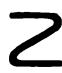
\includegraphics[keepaspectratio]{images/part001_c96515a7.jpg}}

命题 3 的推论表明，域 K 的每个扩张 E 都是包含在 E 中的有限生成扩张的定向并。显然，K 的每个有限次扩张 E 也是有限生成的，因为 E 的一组基（作为 K 上的向量空间）也是 E 在 K 上的一组生成族；我们稍后将看到其逆命题不成立。

